



\begin{exercise}
Find the average rate of change of each function over the indicated interval. Give your answers to two decimal places.

    \begin{parts}
        \item $f(x)=1+x^2$ between $x=1$ and $x=5$.
        
        \item $f(x)=1+x^2$ between $x=-3$ and $x=0$.

        
        \item $\displaystyle g(t)=\frac{1}{t}$ between $t=1$ and $t=3$.

        
        \item $p(x)=2-3x$ between $x=1$ and $x=5$.

        \item $p(x)=2-3x$ between $x=-1$ and $x=2$.
    \end{parts}
\end{exercise}


\begin{solution}
    \begin{parts}
        \item $6$
        \item $-3$
        \item $-1/3$
        \item $-3$
        \item $-3$
    \end{parts}
\end{solution}






\begin{exercise}
In Section 1.3 Exercise~\ref{exercise-1_3-population}, data about the world population, in billions, between the years 2010 and 2018, was given in the table shown below. Use the data to answer the following questions.

\begin{center}\footnotesize
\begin{tabular}{|c|c|c|c|c|c|c|c|c|c|}
\hline Year &2010 & 2011 & 2012 & 2013 & 2014 & 2015 & 2016 & 2017 & 2018
\\\hline Population & 6.957 & 7.041  & 7.126& 7.211  & 7.296 & 7.380 &7.464  & 7.548 & 7.631
\\\hline
\end{tabular}
\end{center}

    \begin{parts}
        \item What was the average rate of change of the world population between 2010 and 2012? Between 2016 and 2018? Give your answers to four decimal places and include units with your answers.

        \item Is there a one-year interval in the time period from 2010 to 2018 during which the average rate of change of the population was negative?
    \end{parts}
\end{exercise}



\begin{solution}
    \begin{parts}
        \item 0.0845 billion people per year; 0.0835 billion people per year
        \item No.
    \end{parts}
\end{solution}






\begin{exercise}
A ball is dropped from a cliff above a lake. The ball's height above the surface of the lake, $h(t)$, in feet, $t$ seconds after the ball is dropped, is given by
\[h(t)=300-16t^2.\]

    \begin{parts}
        \item What is the average rate of change in height $h(t)$ between $t=0$ and $t=3$? Between $t=1$ and $t=4$? Give units with your answers.

        \item Are your answers in part (a) positive or negative? Explain why.
    \end{parts}
\end{exercise}



\begin{solution}
    \begin{parts}
        \item $-48$ feet per second; $-80$ feet per second

        \item negative; the height of the ball is decreasing as time progresses (as it was dropped)
    \end{parts}
\end{solution}







\begin{exercise} In Section 1.2 Exercise~\ref{exercise-1_2-caff}, the graph of a function $C(t)$ (provided again below) was given.

\begin{center}
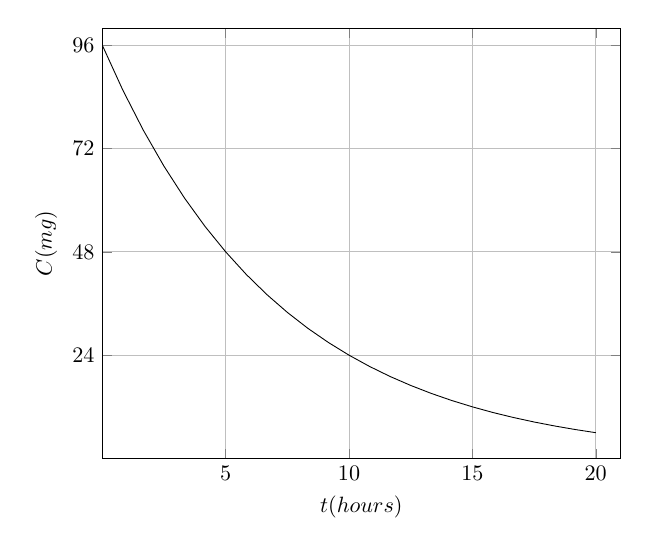
\begin{tikzpicture}[scale=0.8]
\begin{axis}[grid=both,
xmin=0,xmax=21,
ymin=0,ymax=100,
xtick={5,10,...,20},
ytick={24,48,...,96},
% yticklabels={20,40,60,80,100,120},
minor tick={},
xlabel=\(t\text{ (hours)}\), ylabel=\(C\text{ (mg)}\),
x post scale = 1.2,
y post scale = 1.2
]
\addplot[domain=0:20] {96*(1/2)^(x/5)};
\end{axis}
\end{tikzpicture}
\end{center}

\noindent Recall that this graph that models the amount of caffeine, in milligrams, remaining in the body $t$ hours after drinking a cup of coffee. Use the graph to do the following.

%\begin{center}
%\includegraphics[scale=0.6]{graph1-2-12.pdf}
%\end{center}


\begin{parts}
    \item Estimate the average rate of change of $C(t)$ between $t=0$ and $t=5$. Give units with your answer. 

    \item Estimate the average rate of change of $C(t)$ between $t=10$ and $t=15$. Give units with your answer. 

    \item Compare the magnitudes of your answers in (a) and (b). Can you explain the difference by what you see on the graph? 
\end{parts}
\end{exercise}



\begin{solution}
    \begin{parts}
        \item $-9.6$ mg/hr
        \item $-2.4$ mg/hr
        \item The average rate of change from $t = 0$ to $t = 5$ hours is larger than the average rate of change from $t=10$ to $t=15$ hours. It can be seen that the rate at which the amount of caffeine in the bloodstream is changing gets smaller and smaller as time progresses.
    \end{parts}
\end{solution}





\begin{exercise}
The graph of a function $y=f(t)$ is shown below.

\begin{center}
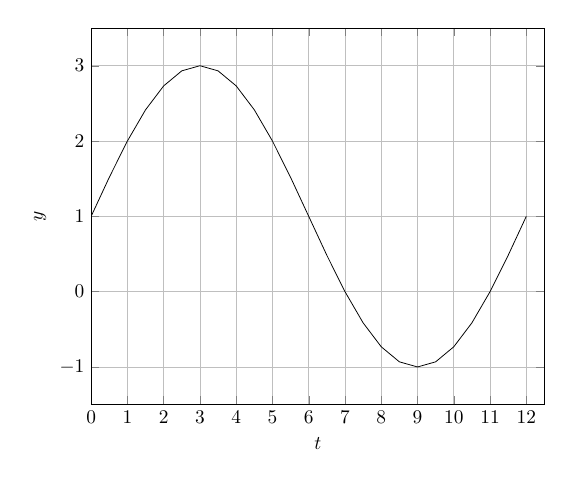
\begin{tikzpicture}[scale=0.7]
\begin{axis}[grid=both,
xmin=0,xmax=12.5,
ymin=-1.5,ymax=3.5,
xtick={0,1,...,12},
ytick={-1,...,3},
minor tick={},
xlabel=\(t\), ylabel=\(y\),
x post scale = 1.2,
y post scale = 1.2
]
\addplot[domain=0:12] {2*sin(2*pi/12*deg(x))+1};
\end{axis}
\end{tikzpicture}
\end{center}

\noindent Without performing any calculations, answer the following questions.

    \begin{parts}
        \item Is the average rate of change of $f(t)$ between  $t=0$ and $t=3$ positive or negative? Explain your answer.

        \item Is the average rate of change of $f(t)$ between  $t=3$ and $t=6$ positive or negative? Explain your answer.

    \end{parts}
\end{exercise}



\begin{solution}
    \begin{parts}
        \item positive since the graph is increasing on this interval
        \item negative since the graph is decreasing on this interval
    \end{parts}
\end{solution}





\begin{exercise}
A person's weight, $W$, in pounds, depends on the number of minutes $m$ of daily exercise. Hence, $W=W(m)$ is a function of $m$. Below is a numerical representation of $W(m)$:
\begin{center}
\begin{tabular}{|c|c|c|c|c|c|c|c|}
\hline $m$ (minutes) & 0 & 20 & 40 & 60 & 80 & 100 & 120
\\\hline $W$ (pounds) & 159 & 152 & 146 & 141 & 137 & 136 & 135.6 
\\\hline
\end{tabular}
\end{center}

    \begin{parts}
        \item Find the average rate of change of $W(m)$ between $m=0$ and $m=40$. Give units with your answer.

        \item Find the average rate of change of $W(m)$ between $m=80$ and $m=120$. Give units with your answer.

        \item Based on your answers and the data in the table, what can you say about the rate of weight loss with increasing amount of exercise?
    \end{parts}


\end{exercise}


\begin{solution}
    \begin{parts}
        \item $-0.325$ pounds/minute
        \item $-0.035$ pounds/minute
        \item The rate of weight loss slows as the daily amount of exercise increases.
    \end{parts}
\end{solution}







\begin{exercise}
Worldwide sales of passenger cars fluctuated between 2012 and 2019\footnote{http://www.oica.net/wp-content/uploads/pc\_sales\_2019.pdf, accessed: 6/30/20}, as can be seen in the table below.
\begin{center}\scriptsize
\begin{tabular}{|c|c|c|c|c|c|c|c|c|c|c|}
\hline Year  & 2010 & 2011 & 2012 & 2013 & 2014 & 2015 & 2016 & 2017 & 2018 & 2019
\\\hline Cars Sold & 55.82 & 57.84 & 60.94 & 63.43 & 65.71 & 66.31 & 69.46 & 70.69 & 68.68 & 64.34 
\\ (millions) & & & & & & & & & &
\\\hline
\end{tabular}
\end{center}

    \begin{parts}
        \item Calculate the average rate of change in sales of passenger cars between the years 2010 and 2017. Give units with your answer.

        \item Calculate the average rate of change in sales of passenger cars between the years 2017 and 2019. Give units with your answer.

        \item In what one-year intervals was the average rate of change negative?
    \end{parts}

\end{exercise}


\begin{solution}
    \begin{parts}
        \item approximately 2.124 million cars sold per year
        \item $-3.175$ million cars sold per year
        \item from 2017 to 2018 and from 2018 to 2019
    \end{parts}
\end{solution}